%-*- coding: utf-8 -*-
\subsection{Renseigner les profils patients}

\begin{figure}[!h]
  \label{diagramme-renseigner-les-profils-patients}
  \centering
  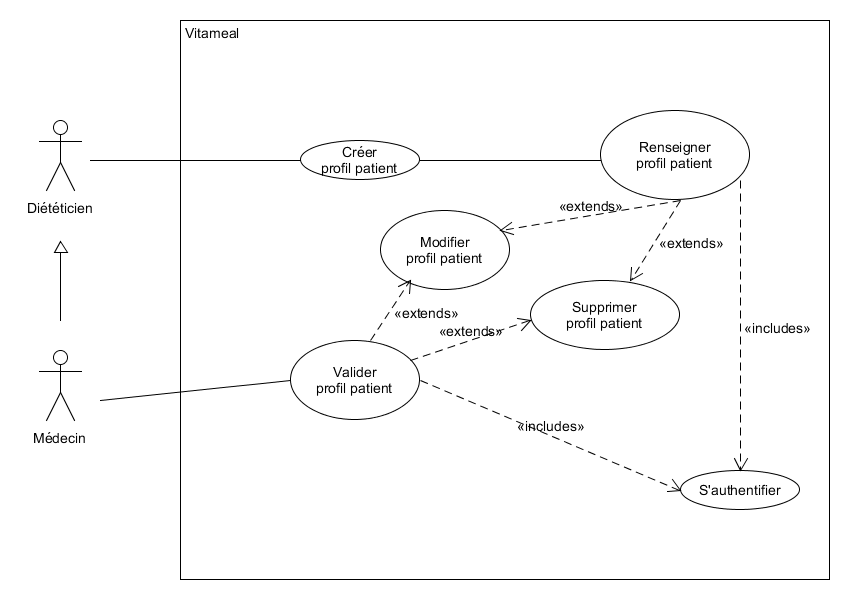
\includegraphics[width=0.9\textwidth]{../../CasDUtilisations/ProfilPatient/ProfilPatient.png}
  \caption{Use case renseigner les profils patients}
\end{figure}

\subsubsection{UC400 - Renseigner profil patient}
\begin{description}
\item [Nom :] Renseigner profil patient
\item [ID :] UC400
\item [Description :] Le diététicien souhaite pouvoir renseigner un profil patient.
\item [Auteur :] Sonia OTHMANI
\item [Date :] 08/05/2017
\item [Acteurs :] Le diététicien
\item [Pré-condition :] L’utilisateur doit être identifié en tant que diététicien (Voir cas d’utilisation \enquote{S’authentifier})
\item [Scénario principal :]
  \begin{enumerate}
  \item Le système affiche une page permettant de créer un profil patient.
  \item L’utilisateur complète les champs relatifs au patient : nom, prénom, date de naissance, pathologies, allergies, régime alimentaire prescrit.
  \item L’utilisateur valide le profil patient.
  \item Le système enregistre le profil patient.
  \end{enumerate}
\item [Scénario alternatif :] Aucun
\item [Post-Conditions :] Le profil patient est créé et enregistré.
\end{description}

\subsubsection{UC401 - Modifier profil patient}
\begin{description}
\item [Nom :] Modifier profil patient
\item [ID :] UC401
\item [Description :] Le diététicien souhaite pouvoir modifier un profil patient.
\item [Auteur :] Sonia OTHMANI
\item [Date :] 08/05/2017
\item [Acteurs :] Le diététicien
\item [Pré-condition :] L’utilisateur doit être identifié en tant que diététicien (Voir cas d’utilisation \enquote{S’authentifier})
\item [Scénario principal :]
  \begin{enumerate}
  \item Le système affiche une liste de profils patients.
  \item L’utilisateur sélectionne la fiche patient à modifier.
  \item L’utilisateur modifie le profil patient.
  \item L’utilisateur valide le profil patient.
  \item Le système enregistre le profil patient modifié.
  \end{enumerate}
\item [Scénario alternatif :] Aucun
\item [Post-Conditions :] Le profil patient est modifié et enregistré.
\end{description}

\subsubsection{UC402 - Supprimer profil patient}
\begin{description}
\item [Nom :] Supprimer profil patient
\item [ID :] UC402
\item [Description :] Le diététicien souhaite pouvoir supprimer un profil patient.
\item [Auteur :] Sonia OTHMANI
\item [Date :] 08/05/2017
\item [Acteurs :] Le diététicien
\item [Pré-condition :] L’utilisateur doit être identifié en tant que diététicien (Voir cas d’utilisation \enquote{S’authentifier})
\item [Scénario principal :]
  \begin{enumerate}
  \item Le système affiche une liste de profils patients.
  \item L’utilisateur sélectionne la fiche patient à supprimer .
  \item L’utilisateur supprime le profil patient.
  \item Le système enregistre la suppression.
  \end{enumerate}
\item [Scénario alternatif :] Aucun
\item [Post-Conditions :] Le profil patient est supprimé
\end{description}
